\documentclass[journal]{IEEEtran}
\usepackage{amsmath,amssymb,amsthm}
\usepackage{graphicx}
\usepackage{booktabs}
\usepackage{tikz}
\usetikzlibrary{positioning,arrows.meta,fit,backgrounds,calc}
\usepackage[hidelinks]{hyperref}
\usepackage{cite}

% generated by make_numbers.py from results/*.json; do not edit
\newcommand{\Rnom}{10}
\newcommand{\RnomS}{0.1667}
\newcommand{\tauNom}{180}
\newcommand{\cNom}{10}
\newcommand{\keNom}{100.00}
\newcommand{\alphaNom}{0.75}
\newcommand{\Ezero}{2.000}
\newcommand{\nDirs}{32}
\newcommand{\bandEps}{0.002}
\newcommand{\babBoxes}{27{,}230}
\newcommand{\babDepth}{40}
\newcommand{\babSec}{1.4}
\newcommand{\eHi}{1.006}
\newcommand{\eLo}{-1.006}
\newcommand{\Ewin}{2.013}
\newcommand{\PbMax}{40.28}
\newcommand{\PgLo}{59.81}
\newcommand{\PgHi}{100.19}
\newcommand{\clipRate}{0.2288}
\newcommand{\clipBinds}{does}
\newcommand{\lbE}{1.404}
\newcommand{\lbP}{40}
\newcommand{\ratioE}{1.43}
\newcommand{\ratioP}{1.007}
\newcommand{\plainProved}{yes}
\newcommand{\plainEwin}{5.700}
\newcommand{\plainPb}{50.28}
\newcommand{\plainRatio}{2.83}
\newcommand{\nSearch}{45}
\newcommand{\nSearchProved}{29}
\newcommand{\sizingRows}{2 & 0.75 & 10 & 900 & 40.28 & 10.064 & 7.018 & 1.43 & 27{,}230 \\
5 & 0.75 & 10 & 360 & 40.28 & 4.026 & 2.807 & 1.43 & 27{,}230 \\
10 & 0.75 & 10 & 180 & 40.28 & 2.013 & 1.404 & 1.43 & 27{,}230 \\
20 & 0.75 & 10 & 90 & 40.28 & 1.006 & 0.702 & 1.43 & 27{,}230 \\
40 & 0.75 & 10 & 45 & 40.28 & 0.503 & 0.351 & 1.43 & 27{,}230 \\}
\newcommand{\famN}{210}
\newcommand{\famRamp}{0.1667}
\newcommand{\famPb}{39.96}
\newcommand{\famB}{-0.002}
\newcommand{\sqN}{330}
\newcommand{\sqEmin}{-1.000}
\newcommand{\sqEmax}{0.995}
\newcommand{\sqPb}{39.96}
\newcommand{\sqB}{-0.002}
\newcommand{\grB}{-0.002}
\newcommand{\grEmin}{-1.000}
\newcommand{\grEmax}{1.000}
\newcommand{\wdPer}{960}
\newcommand{\wdDuty}{0.95}
\newcommand{\wdDepth}{10}
\newcommand{\abN}{140}
\newcommand{\abDrained}{60}
\newcommand{\abPer}{5}
\newcommand{\abDuty}{0.3}
\newcommand{\abDepth}{20}
\newcommand{\abTempty}{17.2}
\newcommand{\abRamp}{199.9}
\newcommand{\noSocDrained}{7}
\newcommand{\noSocEmin}{-1.007}
\newcommand{\oursDrained}{0}
\newcommand{\oursEmin}{-0.931}
\newcommand{\noUpsRamp}{400}
\newcommand{\rpu}{0.0105}
\newcommand{\xpu}{0.0735}
\newcommand{\vUpsLo}{0.9865}
\newcommand{\vUpsHi}{0.9927}
\newcommand{\vUpsDev}{1.35}
\newcommand{\vNoLo}{0.9613}
\newcommand{\vNoHi}{0.9778}
\newcommand{\vNoDev}{3.87}
\newcommand{\vStep}{1.65}
\newcommand{\dVdtMin}{0.165}
\newcommand{\linErrUps}{2.94\times10^{-3}}
\newcommand{\linErrNo}{4.06\times10^{-3}}
\newcommand{\ppExact}{6.7\times10^{-12}}
\newcommand{\ppLin}{4.07\times10^{-3}}
\newcommand{\ppN}{41}


\newtheorem{assumption}{Assumption}
\newtheorem{definition}{Definition}
\newtheorem{problem}{Problem}
\newtheorem{lemma}{Lemma}
\newtheorem{theorem}{Theorem}
\newtheorem{proposition}{Proposition}
\newtheorem{corollary}{Corollary}
\theoremstyle{remark}
\newtheorem{remark}{Remark}

\newcommand{\clip}{\operatorname{clip}}
\newcommand{\sat}{\operatorname{sat}}
\newcommand{\Pmin}{P_{\min}}
\newcommand{\Pmax}{P_{\max}}
\newcommand{\Pbar}{\bar P_b}
\newcommand{\D}{\mathcal{D}}
\newcommand{\Sset}{\mathcal{S}}

\begin{document}

\title{Certified Grid-Side Behavior of an Uninterruptible Power Supply for AI Training Loads}
\author{Sehaj~Singh%
\thanks{S. Singh is with Queens High School for the Sciences, New York, NY, USA.}}

\maketitle

{\small\noindent\bfseries\textit{Abstract:}
Synchronized AI training jobs swing the power of a whole campus between its floor and its peak almost as a step,
and grid operators now ask such loads for guarantees that these swings stay off the grid.
We study a battery and inverter placed between the campus and the grid, run by a deliberately simple grid-side
law: a rate-clipped first-order low-pass of the load plus a saturated loop that restores a \emph{settled} state of
charge. For every measurable load profile with values in a fixed interval, with steps allowed, we prove that the grid
power ramps no faster than a prescribed limit, that the battery stays inside its power rating and energy window,
and that the point-of-common-coupling voltage stays in a band and never steps.
The battery claim rests on a polytopic robust invariant set whose invariance condition is verified by interval
branch-and-bound with outward rounding, and we state precisely why that check implies the claim.
For a public, assumed-parameter campus of $60$ to $100$\,MW and a ramp limit of $\Rnom$\,MW/min, the certificate
needs a $\PbMax$\,MW, $\Ewin$\,MWh battery, within $\ratioE\times$ in energy of a lower bound that we prove holds for
\emph{any} causal controller. Ablations show that a plain ramp-rate limiter drains the same battery on admissible
burst trains, and that restoring the raw state of charge instead of the settled one costs $\plainRatio\times$ more
energy.\par}
\smallskip

{\small\noindent\bfseries\textit{Index Terms:}
Battery energy storage, data centers, robust invariance, interval arithmetic, ramp-rate limits, verification.\par}
\medskip

\section{Introduction}
Large AI training jobs run in lockstep: thousands of accelerators compute together, then communicate or
checkpoint together, so the campus power swings with every training iteration, and the swings grow with job size
\cite{choukse2025}. Grid operators have started to treat such loads as a reliability topic in their own right.
The NERC Large Loads Task Force lists rapid load swings among the risks to frequency and voltage regulation
\cite{nerc2025}; ERCOT has surveyed large electronic loads of $75$\,MW and above about their ride-through behavior
\cite{ercot2025}; and interconnection practice increasingly attaches ramp-rate conditions to such loads
\cite{zahedi2026}. One industrial response is an ``AI UPS'': a medium-voltage battery and inverter that sits between
campus and grid and acts as a firewall in both directions.

A firewall is only useful if its behavior can be guaranteed for \emph{every} load the campus might produce, not only
for the profiles that were simulated. This paper gives such a guarantee for a simple, implementable controller, in the
style of control-theoretic stability results for grid-forming converters \cite{tayyebi2023}: a model with numbered
equations, formal assumptions, and theorems with proofs. The one step that is not closed form, robust invariance of a
battery state set under a saturated nonlinear vector field, is discharged by a computer check whose soundness we argue
explicitly.

\textbf{Contributions.}
(i) A grid-side law that restores the \emph{settled} state of charge $w=e+\tau(P_g-P_{\rm mid})/3600$ rather than the
raw state of charge $e$ (Section~\ref{sec:model}).
(ii) A band lemma (Lemma~\ref{lem:band}) that turns robust invariance of a polytope under measurable inputs into a
finite set of inequalities on boxes, and a sound interval branch-and-bound that proves them
(Proposition~\ref{prop:battery}).
(iii) Ramp, battery and voltage guarantees for every admissible profile (Theorem~\ref{thm:ramp},
Corollary~\ref{cor:voltage}), and a controller-independent lower bound on battery size
(Proposition~\ref{prop:lower}) against which the certified sizes are measured.
(iv) A battery-size versus ramp-limit curve in which every point is certified.

\section{System Model}\label{sec:model}
\begin{figure}[t]
\centering
\resizebox{\columnwidth}{!}{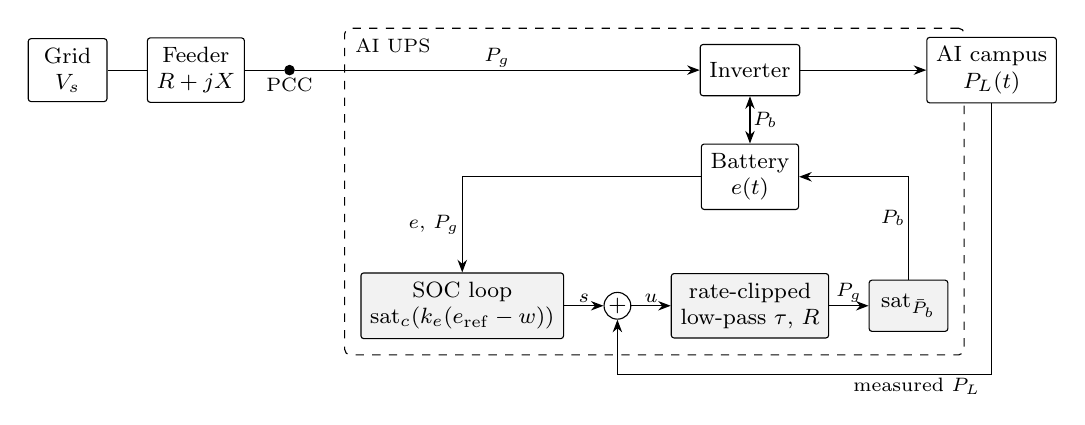
\begin{tikzpicture}[
  font=\footnotesize, >={Stealth[length=1.6mm]}, node distance=4mm and 5mm,
  blk/.style={draw, rounded corners=1pt, minimum height=6.5mm, minimum width=10mm, align=center, fill=white},
  ctl/.style={blk, fill=black!5},
  sum/.style={draw, circle, inner sep=0pt, minimum size=3.4mm},
  lbl/.style={font=\scriptsize, inner sep=1pt}]
  % ---------------- UPS internals first
  \node[blk] (inv) {Inverter};
  \node[blk, below=6mm of inv] (bat) {Battery\\$e(t)$};
  \node[ctl, below=8mm of bat] (lpf) {rate-clipped\\low-pass $\tau$, $R$};
  \node[sum, left=5mm of lpf] (s1) {$+$};
  \node[ctl, left=5mm of s1] (soc) {SOC loop\\$\mathrm{sat}_c(k_e(e_{\mathrm{ref}}-w))$};
  \node[ctl, right=5mm of lpf] (sat) {$\mathrm{sat}_{\bar P_b}$};
  % ---------------- power path
  \node[blk, right=16mm of inv] (load) {AI campus\\$P_L(t)$};
  \coordinate (pccc) at ($(soc.west |- inv)+(-9mm,0)$);
  \node[draw, fill=black, circle, inner sep=1.2pt, label={[lbl]below:PCC}] (pcc) at (pccc) {};
  \node[blk, left=5mm of pcc] (z) {Feeder\\$R+jX$};
  \node[blk, left=5mm of z] (grid) {Grid\\$V_s$};
  \draw (grid) -- (z) -- (pcc);
  \draw[->] (pcc) -- node[lbl, above]{$P_g$} (inv);
  \draw[->] (inv) -- (load);
  \draw[<->] (bat) -- node[lbl, right]{$P_b$} (inv);
  % ---------------- signals
  \draw[->] (soc) -- node[lbl, above]{$s$} (s1);
  \draw[->] (s1) -- node[lbl, above]{$u$} (lpf);
  \draw[->] (lpf) -- node[lbl, above]{$P_g$} (sat);
  \draw[->] (sat.north) |- node[lbl, pos=0.3, left]{$P_b$} (bat.east);
  \draw[->] (load.south) |- ($(s1.south)+(0,-7mm)$) node[lbl, pos=0.6, below]{measured $P_L$} -- (s1.south);
  \draw[->] (bat.west) -| node[lbl, pos=0.75, left]{$e,\,P_g$} (soc.north);
  \begin{scope}[on background layer]
    \node[draw, dashed, rounded corners=2pt, inner sep=2mm, fit=(inv)(bat)(lpf)(soc)(sat),
          label={[lbl, anchor=north west, xshift=1mm, yshift=-1mm]north west:AI UPS}] {};
  \end{scope}
\end{tikzpicture}
}
\caption{Grid, feeder, point of common coupling (PCC), AI UPS and campus. Power flows on the top row; the
controller (shaded) sets the grid-side power $P_g$ from the measured load $P_L$, the stored energy $e$ and $P_g$
itself; the battery supplies the difference $P_b=P_L-P_g$.}
\label{fig:block}
\end{figure}

Fig.~\ref{fig:block} shows the configuration. Powers are in MW, energies in MWh, time in seconds.

\emph{Load.} The campus draws
\begin{equation}\label{eq:load}
P_L(t)\in\D:=[\Pmin,\Pmax],\qquad \Delta P:=\Pmax-\Pmin,
\end{equation}
with no bound on $|dP_L/dt|$. We use $\Pmin=60$, $\Pmax=100$, so $\Delta P=40$, and $P_{\rm mid}=80$.

\emph{Battery power.} By power balance at the UPS, with a power rating $\Pbar$,
\begin{equation}\label{eq:battery}
P_b=\sat_{\Pbar}(P_L-P_g),\qquad P_{\rm grid}=P_L-P_b,
\end{equation}
where $\sat_a(x)=\clip(x,-a,a)$ and $P_b>0$ means discharge.

\emph{State of charge.} With one-way efficiency $\eta\in(0,1]$,
\begin{equation}\label{eq:soc}
\dot e=-\tfrac{1}{3600}\,\varphi(P_b),\qquad
\varphi(p)=\begin{cases}p/\eta,&p\ge 0,\\ \eta p,&p<0,\end{cases}
\end{equation}
with $e$ measured from a reference $e_{\rm ref}=0$. We take $\eta=0.95$ (assumed).

\emph{Controller.} Let $\tau>0$, $R>0$, $c>0$, $k_e>0$ and define the settled state of charge
\begin{equation}\label{eq:w}
w:=e+\tfrac{\tau}{3600}(P_g-P_{\rm mid}).
\end{equation}
The grid-side law is
\begin{equation}\label{eq:ctrl}
\begin{aligned}
\dot P_g&=\clip\!\left(\frac{P_L+s-P_g}{\tau},-R,R\right),\\
s&=\sat_c\big(k_e(e_{\rm ref}-w)\big).
\end{aligned}
\end{equation}
Without the clip and without $s$, \eqref{eq:ctrl} is a first-order low-pass of $P_L$; the clip enforces the ramp limit
by construction; $s$ slowly returns the battery toward its reference. The quantity $w$ is the energy the battery will
hold once $P_g$ has settled at $P_{\rm mid}$ (Lemma~\ref{lem:lpf}(c)); regulating $w$ rather than $e$ stops the SOC
loop from fighting the filter and shrinks the certified energy window by a factor of $\plainRatio$
(Section~\ref{sec:results}).
We parametrize $\tau=\alpha\,\Delta P/R$ and $k_e=c/(\kappa E_0)$ with $E_0:=\tau\Delta P/3600$.

\emph{Feeder voltage.} The PCC is fed from a stiff source $V_s$ through $Z=r+jx$ (per unit, no shunt). For a
grid-side draw $P+jQ$ (per unit) the exact PCC magnitude on the normal operating branch is
\begin{equation}\label{eq:vexact}
\begin{aligned}
V^2&=\tfrac12\Big(A+\sqrt{A^2-4|Z|^2(P^2+Q^2)}\Big),\\
A&=V_s^2-2(rP+xQ),
\end{aligned}
\end{equation}
and its linearization is
\begin{equation}\label{eq:vlin}
V\approx V_s-(rP+xQ)/V_s.
\end{equation}
We use a $69$\,kV, $10$\,km line with $0.05+j0.35\,\Omega$/km on a $100$\,MVA base ($r=\rpu$, $x=\xpu$), $V_s=1$,
the UPS at unity power factor, and, without the UPS, the campus at power factor $0.95$ lagging (all assumed).
An AC power flow in pandapower \cite{thurner2018} on the same feeder agrees with \eqref{eq:vexact} to within
$\ppExact$\,pu at $\ppN$ operating points.

The closed loop \eqref{eq:battery} to \eqref{eq:ctrl} has state $x=(P_g,e)$ and input $P_L$. We write it
$\dot x=f(x,P_L)$.

\begin{assumption}\label{ass:load}
$P_L:[0,\infty)\to\D$ is Lebesgue measurable.
\end{assumption}

\begin{assumption}\label{ass:hw}
The inverter tracks its power reference exactly (no fast current or PLL dynamics), the battery parameters are
constant, the battery can hold every energy in $[e_{\rm lo},e_{\rm hi}]$ given below, and the source behind the
feeder is stiff.
\end{assumption}

Under Assumption~\ref{ass:load}, $f$ is globally Lipschitz in $x$ (it is built from affine maps, clip and the
piecewise-linear $\varphi$) and measurable and bounded in $t$, so for every $x(0)$ there is a unique absolutely
continuous (Carath\'eodory) solution on $[0,\infty)$.

\begin{definition}
A set $\Sset\subset\mathbb{R}^2$ is \emph{robustly forward invariant} if every solution with $x(0)\in\Sset$ and
any $P_L$ satisfying Assumption~\ref{ass:load} has $x(t)\in\Sset$ for all $t\ge 0$.
\end{definition}

\begin{problem}
Given $R$, find controller parameters, a battery rating $\Pbar$, an energy window $[e_{\rm lo},e_{\rm hi}]$ of
smallest width, and a set $\Sset$ of initial states such that for every admissible $P_L$ and every $x(0)\in\Sset$:
(a) $|P_{\rm grid}(t_2)-P_{\rm grid}(t_1)|\le R|t_2-t_1|$; (b) $|P_b(t)|\le\Pbar$ and $e(t)\in[e_{\rm lo},e_{\rm hi}]$;
(c) the PCC voltage stays in $[1-0.05,1+0.05]$ and is Lipschitz in time.
\end{problem}

\section{Main Results}\label{sec:theory}

\subsection{The unsaturated filter in closed form}
\begin{lemma}\label{lem:lpf}
Consider \eqref{eq:ctrl} with $s\equiv 0$ and no clip, i.e.\ $\dot P_g=(P_L-P_g)/\tau$. For every admissible $P_L$:
(a) if $P_g(0)\in\D$ then $P_g(t)\in\D$ for all $t\ge0$;
(b) then $|\dot P_g(t)|\le\Delta P/\tau$ for almost every $t$;
(c) if moreover $\eta=1$ and $|P_L-P_g|\le\Pbar$, then $w(t)=w(0)$ for all $t$.
\end{lemma}
\begin{proof}
(a) At $P_g=\Pmax$, $\dot P_g=(P_L-\Pmax)/\tau\le 0$, and at $P_g=\Pmin$, $\dot P_g\ge0$; for the scalar
absolutely continuous $P_g$ this keeps $P_g\in\D$ (if $P_g(t_1)>\Pmax$, let $t_0$ be the last time before $t_1$ with
$P_g=\Pmax$; on $(t_0,t_1]$ $\dot P_g<0$ a.e., a contradiction). (b) Both $P_L$ and $P_g$ lie in $\D$, so
$|P_L-P_g|\le\Delta P$. (c) $\dot w=\dot e+\tfrac{\tau}{3600}\dot P_g=\tfrac{1}{3600}\big(-(P_L-P_g)+(P_L-P_g)\big)=0$.
\end{proof}

Lemma~\ref{lem:lpf}(b) is the closed-form ramp bound: $\tau\ge\Delta P/R$ suffices. Two things break the closed form.
Losses make $\dot w=-\tfrac{1}{3600}(\varphi(P_b)-P_b)\le0$, so $w$ drifts down forever on any oscillating load
and the battery eventually empties; the SOC loop $s$ is needed to stop that drift, and once it is present $P_g$ can
leave $\D$. The clip lets $\tau<\Delta P/R$, which shrinks the battery, but then $w$ is no longer conserved during
clipped motion. Battery invariance for the full law \eqref{eq:ctrl} is what we certify next.

\subsection{A band lemma for polytopes}
Let $z(x)=\big((P_g-P_{\rm mid})/\Delta P,\ e/E_0\big)$ and, for unit normals $n_k$ and offsets $b_k$,
$k=1,\dots,K$,
\begin{equation}\label{eq:set}
h_k(x)=n_k^\top z(x)-b_k,\quad \Sset=\{x:B(x):=\max_k h_k(x)\le 0\}.
\end{equation}
$B$ is a max of affine functions, i.e.\ a one-hidden-layer ReLU function, and $\Sset$ is a convex polygon. For
$\varepsilon>0$ define the outer bands
$\mathcal{B}_k^\varepsilon=\{x:0\le h_k(x)\le\varepsilon,\ h_j(x)\le\varepsilon\ \forall j\ne k\}$.

\begin{lemma}[band lemma]\label{lem:band}
Suppose that for every $k$,
\begin{equation}\label{eq:band}
\nabla h_k^\top f(x,p)\le 0\quad\forall x\in\mathcal{B}_k^\varepsilon,\ p\in\D.
\end{equation}
Then $\Sset$ is robustly forward invariant.
\end{lemma}
\begin{proof}
Take an admissible $P_L$, a solution with $x(0)\in\Sset$, and suppose $x(t_1)\notin\Sset$ for some $t_1>0$. Let
$t^\ast=\sup\{t\le t_1: x(t)\in\Sset\}$; $\Sset$ is closed, so $x(t^\ast)\in\Sset$ and $t^\ast<t_1$. By continuity
there is $\delta>0$ with $h_j(x(t))\le\varepsilon$ for all $j$ and $t\in[t^\ast,t^\ast+\delta]$, and since
$x(t)\notin\Sset$ for $t\in(t^\ast,t_1]$ there are $t_2\in(t^\ast,t^\ast+\delta]$ and $k$ with
$h_k(x(t_2))>0$. Let $t_3=\sup\{t\le t_2:h_k(x(t))\le0\}\ge t^\ast$, so $h_k(x(t_3))=0$ and
$h_k(x(t))\in(0,\varepsilon]$ on $(t_3,t_2]$. There $x(t)\in\mathcal{B}_k^\varepsilon$, so by \eqref{eq:band}
$\frac{d}{dt}h_k(x(t))=\nabla h_k^\top f(x(t),P_L(t))\le 0$ for almost every $t$. Since $h_k\circ x$ is absolutely
continuous, $h_k(x(t_2))\le h_k(x(t_3))=0$, a contradiction.
\end{proof}

Condition \eqref{eq:band} involves no time and no input signal, only the box $\mathcal{B}_k^\varepsilon\times\D$.
That is what makes it checkable.

\subsection{Sound verification}
For each $k$ the branch-and-bound (BaB) starts from one box in $(P_g,e,P_L)$ that contains
$\mathcal{B}_k^\varepsilon\times\D$ (the bounding box of $\{B\le\varepsilon\}$ padded by $0.05$ in normalized units),
and repeatedly bisects boxes along their widest normalized side. On a box $\mathbf{X}$ it evaluates interval
enclosures $[h_j](\mathbf{X})$ and $[\nabla h_k^\top f](\mathbf{X})$, and discards $\mathbf{X}$ only if
(i) $[h_k]$ misses $[0,\varepsilon]$, or some $[h_j]$, $j\ne k$, lies above $\varepsilon$ (then
$\mathbf{X}\cap\mathcal{B}_k^\varepsilon=\emptyset$), or (ii) the upper end of $[\nabla h_k^\top f](\mathbf{X})$ is
$\le 0$. It reports failure if it finds a box midpoint in the band with positive derivative, or reaches depth
$60$ or its box budget.

\emph{Soundness.} Bisection keeps the live boxes plus the discarded ones a cover of the initial box. Every interval
operation (addition, multiplication, division by a constant, square root) rounds its lower end down and its upper end
up by one unit in the last place; IEEE~754 arithmetic is correctly rounded, so each computed interval contains the
exact real result \cite{moore2009}. $\clip$, $\sat$ and $\varphi$ are monotone, so their images are evaluated
exactly at the endpoints. Hence an interval enclosure is a superset of the true range, and each discard rule is
implied by a true statement about every point of the box. If the BaB terminates with all boxes discarded,
\eqref{eq:band} holds for face $k$.

The vector field in \eqref{eq:band} is evaluated with an unsaturated battery, $P_b=P_L-P_g$. The same BaB proves
$|P_L-P_g|\le\Pbar$ on $\{B\le\varepsilon\}\times\D$, where both fields agree, so \eqref{eq:band} holds for the true
$f$. It also proves the bounds $e_{\rm lo}\le e\le e_{\rm hi}$ and $P_g^{\rm lo}\le P_g\le P_g^{\rm hi}$ on $\Sset$.
Sampling is used only to propose the offsets $b_k$ (faces whose sampled derivative is not strictly negative are pushed
out); it plays no role in the proof.

\begin{proposition}[battery invariance]\label{prop:battery}
Let $R=\Rnom$\,MW/min, $\tau=\tauNom$\,s, $c=\cNom$\,MW, $k_e=\keNom$\,MW/MWh, $\eta=0.95$, and let $\Sset$ be the
$\nDirs$-face polygon \eqref{eq:set} stored in \texttt{results/certificate.json}, with $\varepsilon=\bandEps$.
The BaB proves \eqref{eq:band} for all faces, using $\babBoxes$ boxes, maximum depth $\babDepth$, in
$\babSec$\,s. Consequently, for every admissible $P_L$ and every $x(0)\in\Sset$: $x(t)\in\Sset$, $|P_L(t)-P_g(t)|\le
\PbMax$\,MW, $e(t)\in[\eLo,\eHi]$\,MWh and $P_g(t)\in[\PgLo,\PgHi]$\,MW for all $t\ge0$. With $\Pbar\ge\PbMax$\,MW
the battery power limit never binds, $|P_b(t)|\le\PbMax$\,MW, and the usable energy needed is $\Ewin$\,MWh.
\end{proposition}
\begin{proof}
The BaB terminated with every box discarded for every face, so \eqref{eq:band} holds by the soundness argument above,
and Lemma~\ref{lem:band} gives invariance. The remaining bounds were proved by the same BaB on $\Sset$ (or on
$\{B\le\varepsilon\}\supset\Sset$ for $|P_L-P_g|$) and hold along the trajectory because it stays in $\Sset$.
\end{proof}

\subsection{Ramp and voltage guarantees}
\begin{theorem}[ramp limit]\label{thm:ramp}
Under the hypotheses of Proposition~\ref{prop:battery} with $\Pbar\ge\PbMax$\,MW and an energy window containing
$[\eLo,\eHi]$, for every admissible $P_L$ and every $x(0)\in\Sset$, $P_{\rm grid}(t)=P_g(t)$ and
\[
|P_{\rm grid}(t_2)-P_{\rm grid}(t_1)|\le R\,|t_2-t_1|\qquad\forall t_1,t_2\ge 0 .
\]
\end{theorem}
\begin{proof}
By Proposition~\ref{prop:battery}, $|P_L-P_g|\le\Pbar$ along the trajectory, so the saturation in
\eqref{eq:battery} is inactive and $P_{\rm grid}=P_L-P_b=P_g$; the energy limits are never reached, so no
protection action changes $P_b$. $P_g$ is absolutely continuous with $|\dot P_g|\le R$ a.e.\ by the clip in
\eqref{eq:ctrl}, hence $R$-Lipschitz.
\end{proof}

Without the battery bound the clip alone proves nothing: if the battery saturates or empties, the grid absorbs the
difference $P_L-P_g-P_b$ instantly and sees the load step (Section~\ref{sec:results}).

\begin{corollary}[voltage band]\label{cor:voltage}
Under Theorem~\ref{thm:ramp}, with the UPS at unity power factor and the feeder of Section~\ref{sec:model}, the PCC
voltage \eqref{eq:vexact} satisfies $V(t)\in[\vUpsLo,\vUpsHi]$\,pu, so $|V-1|\le\vUpsDev\%$, for all $t$; and it
changes by at most $\dVdtMin\%$ per minute. The linearization \eqref{eq:vlin} differs from \eqref{eq:vexact} by at
most $\linErrUps$\,pu over the certified range of $P_g$.
\end{corollary}
\begin{proof}
$V$ is a continuous function of $P_g\in[\PgLo,\PgHi]$ (Proposition~\ref{prop:battery}). Covering that interval by
$4000$ subintervals and evaluating \eqref{eq:vexact}, its derivative and $V-V_{\rm lin}$ in outward-rounded interval
arithmetic gives the stated range, a bound $L_V$ on $|dV/dP_g|$, and the linearization error; then
$|V(t_2)-V(t_1)|\le L_V|P_g(t_2)-P_g(t_1)|\le L_VR|t_2-t_1|$ by Theorem~\ref{thm:ramp}.
\end{proof}

\subsection{How small can the battery be?}
\begin{proposition}[lower bound for any controller]\label{prop:lower}
Let any causal controller choose $P_g$ with $|P_g(t_2)-P_g(t_1)|\le R|t_2-t_1|$, and suppose that for every
admissible $P_L$ it keeps $|P_L-P_g|\le\Pbar$ and $e\in[e_{\rm lo},e_{\rm hi}]$ under \eqref{eq:soc}. Then
\[
\Pbar\ge\Delta P,\qquad e_{\rm hi}-e_{\rm lo}\ge\frac{\Delta P^2}{2\eta R\cdot 3600}\ \text{MWh}.
\]
\end{proposition}
\begin{proof}
Fix $\delta\in(0,\Delta P)$ and the profile $P_L\equiv\Pmin$. If $P_g(t)>\Pmin+\delta$ for all $t$, then
$\dot e=\eta(P_g-\Pmin)/3600>\eta\delta/3600$ and $e$ is unbounded, which is excluded. So there is $T$ with
$P_g(T)\le\Pmin+\delta$. Now take the profile equal to $\Pmin$ on $[0,T)$ and $\Pmax$ afterwards. By causality $P_g$
is unchanged on $[0,T]$, and for $t\ge T$, $P_g(t)\le\Pmin+\delta+R(t-T)$. Thus $P_b(T^+)\ge\Delta P-\delta$, and
over $[T,T+(\Delta P-\delta)/R]$ the battery delivers at least $(\Delta P-\delta)^2/(2R)$ MW\,s, drawing at least
$(\Delta P-\delta)^2/(2\eta R\cdot3600)$\,MWh from storage. Since $e(T)\le e_{\rm hi}$ and $e$ stays above
$e_{\rm lo}$, the window is at least that large. Let $\delta\to0$.
\end{proof}

At $R=\Rnom$\,MW/min the bound is $\lbP$\,MW and $\lbE$\,MWh. The certified design uses $\ratioP\times$ the power and
$\ratioE\times$ the energy.

\begin{remark}[scaling in $R$]\label{rem:scaling}
With $\tau=\alpha\Delta P/R$ and $k_e=c/(\kappa E_0)$, the change of variables $z$ in \eqref{eq:set} and time
$t'=tR/\Delta P$ makes the closed loop independent of $R$. So the same normalized polygon is invariant for every $R$,
the certified energy window scales as $1/R$, and $\Pbar$ does not depend on $R$, exactly like the lower bound of
Proposition~\ref{prop:lower}. We nevertheless re-run the BaB at each $R$ of Table~\ref{tab:sizing}, since the
floating-point problem differs.
\end{remark}

\section{Numerical Results}\label{sec:results}
All numbers below are produced by \texttt{run\_all.py} and read from \texttt{results/*.json}.

\emph{Design search.} At $R=\Rnom$\,MW/min we searched $\alpha\in\{0.5,0.6,0.75,0.9,1\}$, $c\in\{3,6,10\}$\,MW and
$\kappa\in\{0.5,0.15,0.05\}$, $\nSearch$ designs, of which $\nSearchProved$ were certified; the others had no
invariant $\nDirs$-face candidate (their offsets diverged), which is a failure of the search, not a proof that no
invariant set exists. The design with the smallest certified window has $\alpha=\alphaNom$, $c=\cNom$\,MW,
$\tau=\tauNom$\,s.

\emph{Sizing curve.} Table~\ref{tab:sizing} and Fig.~\ref{fig:sizing} give the certified battery against the ramp
limit, each row re-certified by BaB at its own $R$, together with the bound of Proposition~\ref{prop:lower}.
\begin{table}[t]
\centering
\caption{Certified battery size versus ramp limit}
\label{tab:sizing}
\setlength{\tabcolsep}{3pt}
\begin{tabular}{rrrrrrrrr}
\toprule
$R$ & $\alpha$ & $c$ & $\tau$ & $\Pbar$ & window & bound & ratio & BaB\\
MW/min & & MW & s & MW & MWh & MWh & & boxes\\
\midrule
\sizingRows
\bottomrule
\end{tabular}
\end{table}
\begin{figure}[t]
\centering
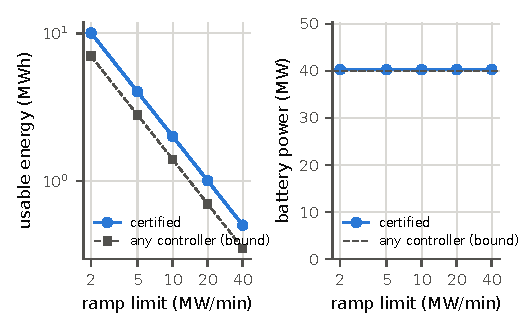
\includegraphics[width=\columnwidth]{../figures/fig_c_battery_vs_ramp.pdf}
\caption{Battery size versus ramp limit. Left: certified usable energy and the lower bound of
Proposition~\ref{prop:lower} (both scale as $1/R$). Right: certified power rating and the bound $\Delta P$.}
\label{fig:sizing}
\end{figure}

\emph{Invariant set.} Fig.~\ref{fig:set} shows $\Sset$ with $\famN$ simulated profiles from the three load families
(square bursts with period $2$ to $30$\,s, duty $0.2$ to $0.8$, depth $10$ to $40\%$; checkpoint dips to idle; random
walks) and a greedy adversary that, at each step, picks the load value that pushes the active face outward fastest.
On all simulated trajectories $\max B=\famB$ (families), $\sqB$ ($\sqN$ square waves with periods up to $960$\,s)
and $\grB$ (adversary), all inside $\Sset$ as the proposition requires. The adversary reaches stored energies in
$[\grEmin,\grEmax]$\,MWh against the certified $[\eLo,\eHi]$\,MWh, so in the energy direction the polygon is close to tight for this design.
The dashed outline is the set certified for the plain loop that restores $e$ instead of $w$, with the same
$(\alpha,c,\kappa)$: its window is $\plainEwin$\,MWh, $\plainRatio\times$ larger.
\begin{figure}[t]
\centering
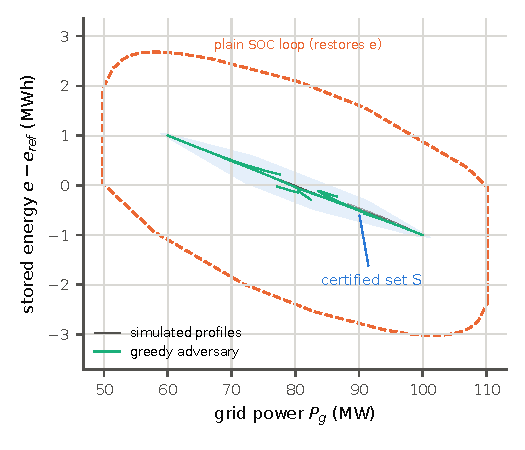
\includegraphics[width=\columnwidth]{../figures/fig_b_invariant_set.pdf}
\caption{Certified invariant set $\Sset$ in the $(P_g,e)$ plane (filled), simulated trajectories (gray), greedy
adversary (green), and the larger set certified for the plain SOC loop (dashed).}
\label{fig:set}
\end{figure}

\emph{Worst-case profiles.} Over the square-wave grid, the deepest discharge came from period $\wdPer$\,s, duty
$\wdDuty$, depth $\wdDepth\%$. Fig.~\ref{fig:worst} shows the three extreme profiles. The grid power is smooth in
every case; the largest simulated battery power was $\sqPb$\,MW against the certified $\PbMax$\,MW.
\begin{figure}[t]
\centering
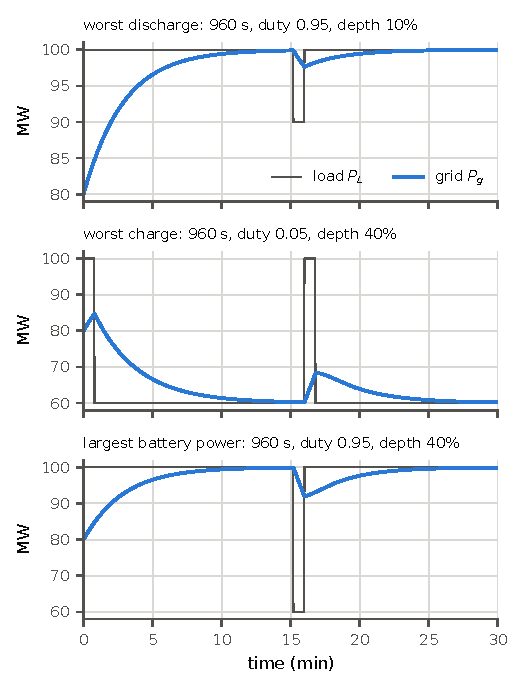
\includegraphics[width=\columnwidth]{../figures/fig_a_worst_profiles.pdf}
\caption{Load (gray) and grid power (blue) on the three extreme square-wave profiles: deepest discharge, highest
charge and largest battery power.}
\label{fig:worst}
\end{figure}

\emph{Voltage.} Fig.~\ref{fig:voltage} compares the PCC voltage on a checkpoint profile. Without the UPS the voltage
stays in $[\vNoLo,\vNoHi]$\,pu, inside the $5\%$ band, but a full load step moves it by $\vStep\%$ instantly. With
the UPS it stays in $[\vUpsLo,\vUpsHi]$\,pu and moves at most $\dVdtMin\%$ per minute
(Corollary~\ref{cor:voltage}). On this assumed stiff feeder the gain is the removal of steps, not the band itself.
The linearization error over the no-UPS range is at most $\linErrNo$\,pu; against pandapower the linear model is
off by at most $\ppLin$\,pu.
\begin{figure}[t]
\centering
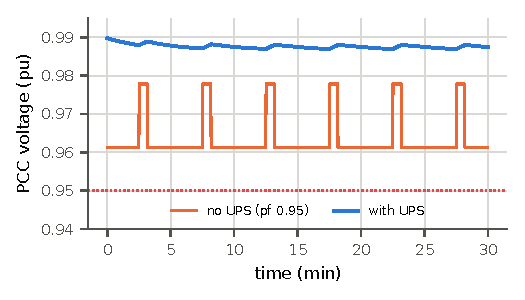
\includegraphics[width=\columnwidth]{../figures/fig_d_pcc_voltage.pdf}
\caption{PCC voltage without the UPS (campus at power factor 0.95) and with the certified UPS, checkpoint profile
with a 40\,s dip to idle every 300\,s. Dotted: lower edge of the $5\%$ band.}
\label{fig:voltage}
\end{figure}

\emph{Ablations.} Without a UPS the grid sees $P_L$ itself: a $40$\,MW step within one $0.1$\,s simulation sample,
$\noUpsRamp$\,MW/s at that resolution and unbounded in the limit, against $R=\RnomS$\,MW/s.
A classic ramp-rate limiter ($\dot P_g=\clip((P_L-P_g)/1\,\mathrm{s},-R,R)$, no SOC loop) given the same certified
battery drained it on $\abDrained$ of $\abN$ burst trains from the brief's family within $2$\,h; the fastest was
period $\abPer$\,s, duty $\abDuty$, depth $\abDepth\%$, empty after $\abTempty$\,min, after which the grid sees ramps
of $\abRamp$\,MW/s (Fig.~\ref{fig:ablation}). The reason is the asymmetry of short bursts: during a short high phase
the limiter cannot catch up, so the battery supplies most of every burst and recovers little in between. The certified
filter with its SOC loop removed drained the battery on $\noSocDrained$ of the same profiles, while the certified
controller drained it on $\oursDrained$, with minimum stored energy $\oursEmin$\,MWh.
\begin{figure}[t]
\centering
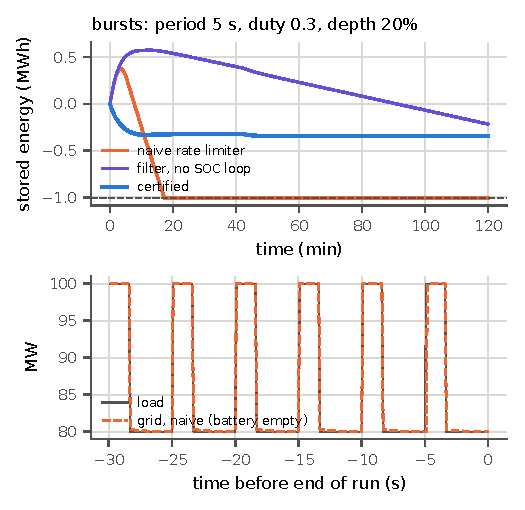
\includegraphics[width=\columnwidth]{../figures/fig_e_ablation.pdf}
\caption{Ablation on an admissible burst train. Top: stored energy for the naive rate limiter, the filter without
SOC loop, and the certified controller; dashed: certified lower energy limit. Bottom: last 30\,s of load and grid
power for the naive limiter, after its battery is empty: the grid sees every load step.}
\label{fig:ablation}
\end{figure}

\section{Related Work}
Stability guarantees for grid-forming converters are typically given as theorems on a stated model, as in hybrid angle
control \cite{tayyebi2023}; for the broader low-inertia context see \cite{milano2018}. Our object is simpler (a
power-reference law, not a converter) but our guarantee is for every input signal in a set, so the tool is set
invariance \cite{blanchini1999,blanchini2008} rather than Lyapunov stability. Barrier certificates
\cite{prajna2004,ames2019} prove safety with a function whose sublevel set is invariant; our $B$ is such a function,
in max-of-affine form, verified by interval analysis \cite{moore2009} instead of sum-of-squares programming.
The load side is documented in \cite{choukse2025}, which characterizes power swings of large training jobs and
discusses mitigations framed by utility specifications such as ramp-rate limits. The grid side is in the NERC white paper
\cite{nerc2025}, the ERCOT survey \cite{ercot2025}, and a survey of interconnection practice \cite{zahedi2026}.

\section{Limitations}
This is a public, assumed-parameter model. None of the parameters come from ON.energy hardware or data, and the
controller is ours, not a vendor's. The proof covers the averaged power model only: no inverter current or PLL
dynamics, no switching, no faults, no ride-through events, no protection, no communication delay or measurement
noise on $P_L$, no battery aging, temperature or state-dependent efficiency. The load set allows any measurable profile
in $[60,100]$\,MW, but not excursions outside it (for example a full trip to zero). The feeder is a stiff source
behind one line; real PCC voltage depends on the rest of the network and on the campus's own reactive power.
The certified set is a $\nDirs$-face polygon found by a heuristic search over a small design grid, so the sizes are
upper bounds for this controller family, and the gap to the lower bound of Proposition~\ref{prop:lower} may be
partly due to the template rather than the controller. Finally, the BaB proof is only as trustworthy as its
implementation; the code is small and tested, but it has not been formally verified.

\section{Conclusion}
A low-pass with a rate clip and a saturated loop on the settled state of charge is enough to give a provable firewall
between an AI campus and the grid: bounded ramp, bounded battery power and energy, and a step-free PCC voltage, for
every admissible load profile. The battery it needs is within a small factor of what any controller needs, and the
certificate makes clear which piece buys which property.

\begin{thebibliography}{10}
\bibitem{choukse2025}
E.~Choukse \emph{et al.}, ``Power stabilization for AI training datacenters,'' arXiv:2508.14318, 2025.
\bibitem{nerc2025}
NERC Large Loads Task Force, ``Characteristics and risks of emerging large loads,'' white paper, North American
Electric Reliability Corporation, Jul. 2025.
\bibitem{ercot2025}
ERCOT, ``Large load survey and request for information of voltage ride-through capabilities,'' Market Notice
M-B062325-01, Jun. 2025.
\bibitem{zahedi2026}
R.~Zahedi, A.~Zamani, and R.~Anilkumar, ``Best practices for large load interconnections: A North American perspective
on data centers,'' arXiv:2601.12686, 2026.
\bibitem{tayyebi2023}
A.~Tayyebi, A.~Anta, and F.~D\"orfler, ``Grid-forming hybrid angle control and almost global stability of the DC-AC
power converter,'' \emph{IEEE Trans. Autom. Control}, pp.~3842--3857, 2023. Preprint: ``Hybrid angle control and
almost global stability of grid-forming power converters,'' arXiv:2008.07661.
\bibitem{milano2018}
F.~Milano, F.~D\"orfler, G.~Hug, D.~J. Hill, and G.~Verbi\v{c}, ``Foundations and challenges of low-inertia systems,''
in \emph{Proc. Power Systems Computation Conf. (PSCC)}, 2018.
\bibitem{blanchini1999}
F.~Blanchini, ``Set invariance in control,'' \emph{Automatica}, vol.~35, no.~11, pp.~1747--1767, 1999.
\bibitem{blanchini2008}
F.~Blanchini and S.~Miani, \emph{Set-Theoretic Methods in Control}. Boston, MA, USA: Birkh\"auser, 2008.
\bibitem{prajna2004}
S.~Prajna and A.~Jadbabaie, ``Safety verification of hybrid systems using barrier certificates,'' in \emph{Hybrid
Systems: Computation and Control (HSCC)}, 2004, pp.~477--492.
\bibitem{ames2019}
A.~D. Ames, S.~Coogan, M.~Egerstedt, G.~Notomista, K.~Sreenath, and P.~Tabuada, ``Control barrier functions: Theory
and applications,'' in \emph{Proc. European Control Conf. (ECC)}, 2019, pp.~3420--3431.
\bibitem{moore2009}
R.~E. Moore, R.~B. Kearfott, and M.~J. Cloud, \emph{Introduction to Interval Analysis}. Philadelphia, PA, USA: SIAM,
2009.
\bibitem{thurner2018}
L.~Thurner \emph{et al.}, ``pandapower: An open-source Python tool for convenient modeling, analysis, and optimization
of electric power systems,'' \emph{IEEE Trans. Power Syst.}, vol.~33, no.~6, pp.~6510--6521, 2018.
\end{thebibliography}

\end{document}
